\begin{frame}
\frametitle{Problems arising during packet capturing}
%\textbf{Problems arising during packet capturing:}\newline
\begin{itemize}
	\item High bit rates and packet rates
		\begin{itemize}
			\item [$\Rightarrow$] \textbf{\textcolor{red}{high CPU load and packet loss}}
		\end{itemize}
\end{itemize}

\ifthenelse{\boolean{SUMMIT}}{}{
\begin{figure}[H] 
	\subfigure{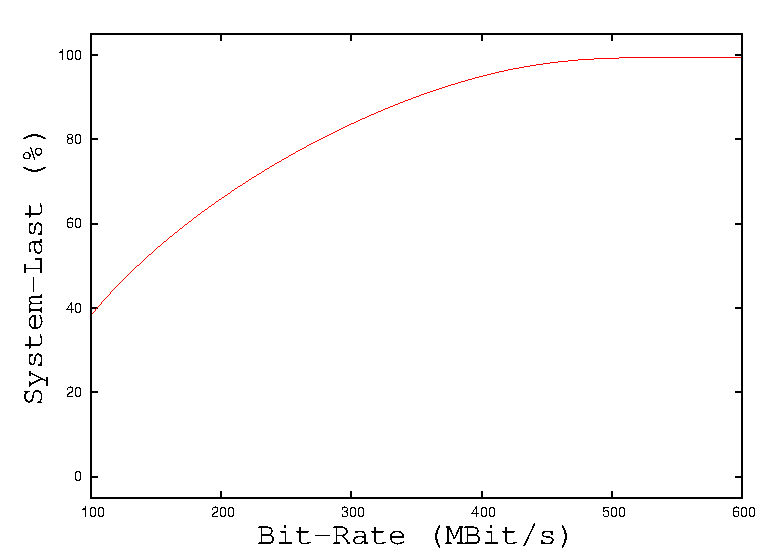
\includegraphics [width=0.45\textwidth]{plots/sysload_generic_slide}}
	\subfigure{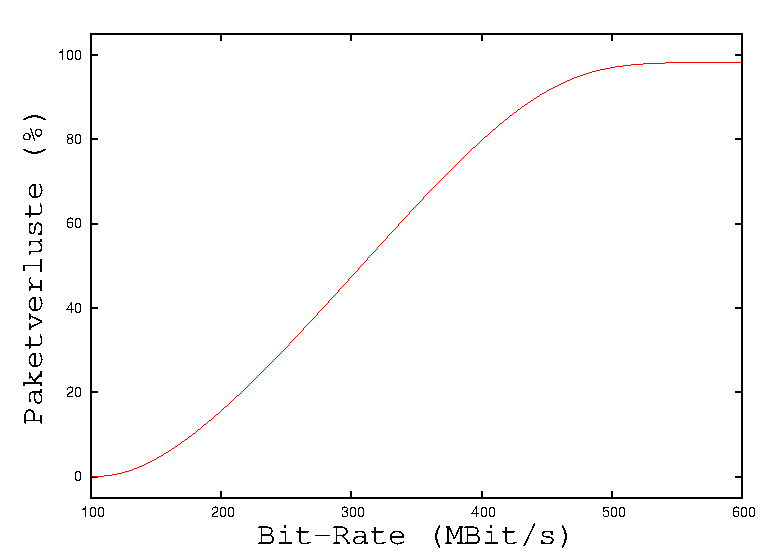
\includegraphics [width=0.45\textwidth]{plots/pktlos_generic_slide}}
	\caption{Capturing 64-Bytes packets. (Bezier curves)}
\end{figure}
\end{frame}

\begin{frame}
\frametitle{The reason of the Problems}
}
\ifthenelse{\boolean{SUMMIT}}{
}{
\textbf{Inefficiency of standard capturing software}
}
	\begin{itemize}
	\item ``expensive'' operations in terms of CPU cycles: 
		\begin{itemize}
			\item Memory allocations
			\item Data copy operations
			\item System calls
			\item etc\ldots\newline
		\end{itemize}
% \begin{small}
% 	\item [$\Rightarrow$] probably the capturing software for FreeBSD was
% 		developed at a time when  network data-rates were low enough relative
% 		to hardware processing resources such that capturing loss problems did
% 		not arise?
% \end{small}
	\end{itemize}

\end{frame}

\ifthenelse{\boolean{SUMMIT}}{
\subsection*{Disadvantages of standard capturing software}
\begin{frame}
\frametitle{Disadvantages of Standard Packet Capturing Stack}
\begin{itemize}
	\item<1-> Memory allocations
		\begin{itemize}
			\item<1-> For each new received packet a new \emph{mbuf} 
				is allocated\newline
		\end{itemize}


	\item<2-> Too many packet copies
		\begin{itemize}
\ifthenelse{\boolean{SUMMIT}}{
			\item<2-> DMA: $Controller \Rightarrow RAM$
			\item<2-> BPF: $RAM \Rightarrow RAM (BPF\ Buffer)$
			\item<2-> read(2): $RAM \Rightarrow RAM (Userspace\ Buffer)$\emph{(*)}\newline
}{
			\item<2-> DMA: $FIFO \Rightarrow Packet\ Buffer$
			\item<2-> $Packet\ Buffer \Rightarrow BPF\ Buffer$
			\item<2-> $BPF\ Buffer \Rightarrow Userspace\ Buffer$\emph{(*)}\newline
}
		\end{itemize}

	\item<3-> System calls
		\begin{itemize}
			\item<3-> User-space application receives the packets using read(2)\emph{(*)}
			\item<3-> Saving packets to the hard disk\newline
		\end{itemize}

\end{itemize}
\begin{tiny}
\emph{(*)} Using Zero-Copy BPF eliminates the last copy and system call
\end{tiny}
\end{frame}

} {}
